\documentclass[jcp,groupaddress]{revtex4-1}
% graphical packages
\usepackage{amsthm}
\usepackage{float}
\usepackage{multirow}
\usepackage{graphicx}
\usepackage{caption}
\usepackage{subcaption}
% mathematical packages
\usepackage{amsmath}
\usepackage{amssymb}
\usepackage{mathtools}
\usepackage{bm}
% Other packages
\usepackage[titletoc,toc,title]{appendix}
% custom commands
\DeclareMathOperator{\sign}{sgn}
\newtheorem{theorem}{Theorem}
\newtheorem{definition}{Definition}
\newtheorem{corollary}{Corollary}[theorem]
\newcommand{\dotproduct}[2]
{
#1 \cdot #2
}
\newcommand{\eq}{\begin{equation}}
\newcommand{\qe}{\end{equation}}
\DeclareMathOperator{\erf}{Erf}
\DeclareMathOperator{\erfc}{Erfc}
\DeclareMathOperator{\erfi}{Erfi}
\newcommand{\obrt}{\frac{1}{\sqrt{2}}}
\newcommand{\lp}{\left(}
\newcommand{\rp}{\right)}
\newcommand{\diff}{\mathrm{d}}
\newcommand{\rr}{\mathbf{r}}
\newcommand{\ham}{\hat{\mathcal{H}}}
\newcommand{\p}{\hat{p}}
\newcommand{\num}{\hat{N}}
\newcommand{\fact}[1]{#1!}
\newcommand{\abs}[1]{\vert #1\vert}
\newcommand{\bra}[1]{\langle #1 \vert}
\newcommand{\ket}[1]{\vert #1 \rangle}
\newcommand{\commutator}[2]
 {
 [ #1 ,  #2
  ]
}
\newcommand{\eqnref}[1]{
Eq.(\ref{#1})
}
\newcommand{\threepartdef}[6]
{
	\left\{
		\begin{array}{lll}
			#1 & \mbox{if } #2 \\
			#3 & \mbox{if } #4 \\
			#5 & \mbox{if } #6
		\end{array}
	\right.
}

\newcommand{\ie}{\emph{i.e. }}
\newcommand{\viz}{\emph{viz.}}
\newcommand{\via}{\emph{via }}

\begin{document}
\title{On non-local response functions of quantum harmonic oscillator and their application in theory of van der Waals interactions}
\maketitle
\author{Jan Hermann}
\author{M. Sadhukhan}
\author{Alexandre Tkatchenko}
\date{}



% \section{Definitions and important formulae}
% \begin{itemize}
%  \item{\bf Fourier transform}\\

%     We will use the unitary symmetric Fourier transform pairs
%      \begin{eqnarray*}
%       \mathcal{F}[f] \coloneqq \hat{f}(\boldsymbol{\omega})&=& \frac{1}{(2\pi)^{n/2}}\int_{\mathbf{R}^{n}}f(\rr)e^{i\boldsymbol{\omega}.\rr}\diff \rr \\
%      \mathcal{F}^{-1}[\hat f] \coloneqq  f(\rr)&=& \frac{1}{(2\pi)^{n/2}}\int_{\boldsymbol{\omega}^{n}}\hat{f}(\boldsymbol{\omega})e^{-i\boldsymbol{\omega}.\rr}\diff \boldsymbol{\omega}
%      \end{eqnarray*} 
%  \item{\bf Delta function}\\

%   We will use the following representation of the Delta function to be consistent with Fourier transform convention:\\
% \begin{equation*}
%  \delta(x-x')= \frac{1}{2\pi} \int_{-\infty}^{\infty}  e^{ik(x-x')}\diff k
% \end{equation*}

% \item{\bf Convolution theorem for FT}\\

%  Suppose $\hat{f} = \mathcal{F}[f]$ and $\hat{g} = \mathcal{F}[g]$. Then the convolution of $\hat{f}$and  $\hat{g}$ is related to $f$ and $g$ by 
% \begin{equation*}
% \hat{f}*\hat{g} \coloneqq \frac{1}{\sqrt{2\pi}} \int_{-\infty}^{\infty} \diff k' \, \hat{f}(k-k')\hat{g}(k')= \frac{1}{\sqrt{2\pi}}  \int_{-\infty}^{\infty} e^{ik x} f(x) g(x) \diff x
% \end{equation*}
% \item{\bf Integration of function}\\
%  For an FT pair $(f,\hat{f})$,
% \begin{equation*}
% \hat{f}(0) = \frac{1}{\sqrt{2\pi}} \int_{-\infty}^{\infty} f(x) \diff x
% \end{equation*}

% \item{\bf Time-scaling of FT}\\

% If $g(x) = f(a x)$ then 

%  \begin{equation*}
% \hat{g}(x) = \frac{1}{\abs{a}}\hat{f}(\frac{x}{a})
% \end{equation*}

% \item{\bf Duality of FT}\\

% \begin{equation*}
% \mathcal{F}[f](-k) =\mathcal{F}^{-1}[f](k)
% \end{equation*}
% \item{\bf Error function}\\
%   \begin{equation*}
% \erf(x) = \frac{2}{\sqrt{\pi}}\int_{0}^{x}  e^{-t^{2}} \diff t =  \frac{1}{\sqrt{\pi}}\int_{-x}^{x}  e^{-t^{2}} \diff t 
% \end{equation*}
% \item{\bf Complimentary error function}\\
%   \begin{equation*}
% \erfc(x) = \frac{2}{\sqrt{\pi}}\int_{x}^{\infty}  e^{-t^{2}} \diff t = 1-\erf(x)
% \end{equation*}

 

% \end{itemize}
\section{Introduction}
\section{Polarizability and other response functions}
The polarizability describes a systems ability to be deformed in response to the perturbations. In case of electronic systems, this perturbations are the electric and/or magetic fields. We will concentrate here only on the electric fields. The perturbing electric field can come from the external as well as internal fluctuations of electric charges. The \emph{fluctuation-dissipation theorem}\cite{langreth1977} ascertains that the nature of the electronic response for both cases are same.  
\subsection{Polarizability}
When a symmetric or spherical electron density gets deformed asymetry is created. As a result, in a simplest case, a dipole is created. It is obvious to that stronger electric field will create larger dipole moment. 
\begin{equation}
 \mu = \alpha E
\end{equation} 
  In general, if both the time-dependent electric field and the electronic response is anisotropic in space, we can write,
\eq
\boldsymbol{\mu} (t)= \int_{0}^{t} \diff t' \dotproduct{\boldsymbol{\alpha}(t,t')}{\mathbf{E}(t')}\Theta(t-t')
\qe
 or,
\eq
\mu(\rr, t) =  \int_{0}^{t} \diff t' \int_{V} \diff \rr' \alpha(\rr,\rr',t, t' )E(\rr', t')\Theta(t-t')
\qe
where the step function $\Theta(t-t')$ assures causality.\\
\subsection{Density response function}
As its name implies, this response function measures the spatio-temporal responses of electronic density under the influence of perturbing electric field. Consider a slight change in the external scalar potential (the source can be anything from internal density fluctuation to external electric fields) $\Delta \phi(\mathbf{r}, t)$ such that the electric field changes by the amount of 
\eq
 \Delta \mathbf{E}(\mathbf{r}, t) = \nabla(\Delta \phi(\mathbf{r}, t))
\qe
In response, the electron density gets deformed by an amount
\eq
\Delta \rho(\mathbf{r}, t) = \int_{V} \diff \mathbf{r}' \int_{0}^{\infty} \diff t' \Theta(t - t') \chi(\mathbf{r},\mathbf{r}', t', t) \Delta \phi(\mathbf{r}', t') 
\qe
where the step function, again assures causality. The kernel $\chi(\rr, \rr', t, t')$ is the density-density response function. Interestingly, this is actually a Green's function and can be connected to density matrix of the free theory.  Note that due to causality condition and for system with conserved energy, we can argue that $\chi$ only depends on the absolute value of time difference $\abs{t-t'}$. In that case we can rewrite,
\eq
\Delta \rho(\mathbf{r}, t) = \int_{V} \diff \mathbf{r}' \int_{0}^{\infty} \chi(\mathbf{r},\mathbf{r}', t) \Delta \phi(\mathbf{r}', 0).
\qe

\par The response properties of an electronic fragment can be calculated \via the so-called Adler-Wiser sum (AWS)
\eq\label{awsum}
\chi(\rr, \rr', i u) = \sum_{j,k}\frac{(f_{j}-f_{k})\psi_{j}^{*}(\rr)\psi_{j}(\rr')\psi_{k}^{*}(\rr)\psi_{k}(\rr')}{\epsilon_{j}-\epsilon_{k}+ i u}
\qe
where $f_{j}$ and $\epsilon_{j}$ represent occupation number and energy of the orbital $\psi_{j}$. Also note that frequency $u$ is expressed in the unit of $\hbar$. As a result for any dimensional analysis $u \rightarrow u \hbar$\\

The straightforward way of defining response function is,
\eq
 \chi(\rr,\rr',t,t') = \frac{\delta n(\rr,t)}{\delta \phi(\rr',t')}
\qe 
We may need to consider this straight route as well for some problem. It is a possibility that  AWS in Eq.~\eqref{awsum} may not be valid in this form for bosons. 
\section{Response function for a classical 1D SHO}
We are going to examine the response of a classical SHO. We must first clarify the definitions. \\
Suppose the equation of motion of a dynamical system is 
\eq
\ddot{x}+ g(x, \dot{x})=0
\qe
We want to know how it responds to an external accelaration $a(x,t)$. Therefore we want to know the behavior for 
\eq
\ddot{x}+ g(x, \dot{x})=a(x,t)
\qe
The answer can be worked out interms of Green's function $G(t, t')$. If the dynamics is invariant under time translation symmetry, which is the case most often, then we can say $G(t, t')\equiv G( t-t') \equiv G(t)$
\eq
x(t) = \int_{0}^{\infty}\diff t' G(t-t') a(t')\Theta(t-t')
\qe
Note here that the causality demands $t> t'$ and the Haviside step function assures that. We also know that the Green's function is the solution of the equation
\eq
\ddot{G}(t-t')+ g(G( t-t'), \dot{G}(t-t')) = \delta(t-t')
\qe
For a single 1D damped, driven classical SHO the equation of motion is 
\eq
\ddot{x} + \omega_{0}^{2}x -\gamma \dot{x} = a(t)
\qe
a(t) is the force and $\gamma$ provides damping.  The Green's function is the solution of
\eq
\ddot{G}(t)-\gamma \dot{G}(t)+ \omega_{0}^{2}G(t) = \delta(t)
\qe
Taking the inverse Fourier transform for $(t \to \omega)$, 
\eq
-\omega^2 \tilde{G}(\omega)-i\omega \gamma \tilde{G}(\omega)+ \omega_{0}^{2}\tilde{G}(\omega) = 1
\qe
or
\eq
\tilde{G}(\omega) = \frac{1}{\omega_{0}^{2}-\omega^{2}-i\omega \gamma}
\qe
Replacing $\omega \to i \omega$ 
\eq
\tilde{G}(i\omega) = \frac{1}{\omega_{0}^{2}+\omega^{2}+\omega \gamma}
\qe
Therefore the time domain function is 
\eq
\hat{G}(t) = \mathcal{F}[\tilde{G}] = \frac{1}{\sqrt{2\pi}}\int_{-\infty}^{\infty} \diff \omega \frac{e^{i\omega t}}{\omega_{0}^{2}+\omega^{2}+\omega \gamma}
\qe
For non-damped oscillator ($\gamma =0$),
\eq
\hat{G}(t) = \frac{1}{\sqrt{2\pi}}\int_{-\infty}^{\infty} \diff \omega \frac{e^{i\omega t}}{\omega_{0}^{2}+\omega^{2}}
\qe 
or,
\eq
\hat{G}(t) = \frac{e^{-\omega_{0} \abs{t}}}{2\omega_{0}} 
\qe 
\section{A brief sketch about the Adler-Wise sum}

 Adler-Wiser sum (Eq.\eqref{awsum}) gives an expression for dielectric constant of a solid in terms of its SCF eigenspecta. 


\section{Response properties of a single harmonic oscillator}
 \subsection{Quantum mechanics of harmonic oscillator}
  We can calculate the response function \via \eqnref{awsum}. This is going to be a brute force method.\\
We realize that the wave function of a 3D oscillator is 
\eq\label{shof}
 \psi_{\mu}(\rr) = \frac{1}{\sqrt{2^{\mu}\fact{\mu_{x}}\fact{\mu_{y}}\fact{\mu_{z}}}}\lp\frac{m \omega_{0}}{\pi} \rp^{3/4}
e^{\frac{m \omega_{0}\rr^{2}}{2}}H_{\mu_{x}}(\sqrt{m \omega_{0}}x)H_{\mu_{y}}(\sqrt{m \omega_{0}}y)H_{\mu_{z}}(\sqrt{m \omega_{0}}z)
\qe
for an oscillator having mass $m$ and natural frequency $\omega_{0}$ with quanta $\mu = \mu_{x} + \mu_{y} + \mu_{z}$.The energy is 
\eq\label{3den}
 \epsilon_{\mu} = \left(\mu + \frac{3}{2}\right)\hbar \omega_{0}
\qe
The degeneracy of the state is 
\eq
 g_{\mu} = \binom{\mu+2}{2}
\qe
\subsection{Response property of 1D SHO}
  We will start by calculating the response function of 1D SHO \via Eq.~\eqref{awsum}. If the oscillator is in ground state, its occupation number is defined as
\eq
 f_{\mu} = \delta_{\mu 0}
\qe
Its energy
\eq
 \epsilon_{\mu} = \left( \mu + \frac{1}{2}\right)\hbar \omega
\qe
and wavefunction 
\eq
\psi_{\mu}(x) = \left(\frac{m \omega}{\pi \hbar} \right)^{1/4} \frac{1}{\sqrt{2^{\mu}\fact{\mu}}}e^{-\frac{m\omega x^2}{2\hbar}}H_{\mu}\left(\sqrt{\frac{m\omega}{\hbar}}x\right)
\qe
is distinguished by the natural frequency $\omega$ and mass $m$.  Plugging everything in Eq.~\eqref{awsum} and realizing that for $\mu=\nu=0$, $f_{\mu}-f_{\nu} = 0$, we obtain
\eq
 \chi(x, x', i u)= \sum_{\nu=1}^{\infty}\frac{(1-\delta_{\nu 0})\rho_{0}(x, x')\rho_{\nu}(x, x')}{-\nu \hbar \omega + i u}+ \sum_{\mu=1}^{\infty}\frac{(\delta_{\mu 0}-1)\rho_{0}(x, x')\rho_{\mu}(x, x')}{\mu \hbar \omega + i u}
\qe
The first term in RHS is for $\mu = 0$ and the second term is for $\nu = 0$. Since $\mu$ and $\nu$ are dummy indices, we can rewrite the expression as,
\eq
 \chi(x, x', i u)= \sum_{\mu=1}^{\infty}\rho_{0}(x, x')\rho_{\mu}(x, x')\left( \frac{1}{iu-\mu \hbar \omega} -\frac{1}{iu + \mu \hbar \omega}\right)
\qe
where the density matrix for $\mu$-th state
\eq
\rho_{\mu}(x, x') = \left(\frac{m \omega}{\pi \hbar} \right)^{1/2} \frac{1}{2^{\mu}\fact{\mu}}e^{-\frac{m\omega x^{2}}{\hbar}}H_{\mu}\left(\sqrt{\frac{m \omega}{\hbar}}x \right)H_{\mu}\left(\sqrt{\frac{m \omega}{\hbar}}x' \right)
\qe
With a little algebra we obtain
\eq\label{chi_u}
 \chi(x, x', i u)= -2\rho_{0}(x, x') \sum_{\mu=1}^{\infty}\rho_{\mu}(x, x')\left( \frac{\mu \hbar \omega }{u^2+(\mu \hbar \omega)^{2}} \right)
\qe
Now we will Fourier transform $\chi$ to obtain
\eq
\hat{\chi}(x, x', t)=-\sqrt{2\pi}\rho_{0}(x, x') \sum_{\mu=1}^{\infty}\rho_{\mu}(x, x')e^{-\mu \hbar \omega \abs{t}}
\qe
Again with little more algebra e obtain,
\eq
\hat{\chi}(y, y', t)=-\sqrt{2\pi}\left( \frac{m \omega}{\pi \hbar}\right) e^{-(y^2+{y'}^2)} \sum_{\mu=1}^{\infty}\frac{H_{\mu}(y)H_{\mu}(y')}{2^{\mu}\fact{\mu}}e^{-\mu \hbar \omega \abs{t}}
\qe
where $y = \sqrt{m \omega/\hbar}x$
We now can write,
\eq
\hat{\chi}(y, y', t)=-\sqrt{2\pi}\left( \frac{m \omega}{\pi \hbar}\right) e^{-(y^2+{y'}^2)} \sum_{\mu=1}^{\infty}\frac{H_{\mu}(y)H_{\mu}(y')}{2^{\mu}\fact{\mu}}\zeta^{\mu}
\qe
where 
\eq
 \zeta = e^{-\hbar \omega \abs{t}}  
\qe
We realize that 
\eq
0 \le \zeta \le 1; \forall t
\qe
Therefore, 
\eq
\hat{\chi}(y, y', t)=-\sqrt{2\pi}\left( \frac{m \omega}{\pi \hbar}\right) e^{-(y^2+{y'}^2)} \left( \sum_{\mu=0}^{\infty}\frac{H_{\mu}(y)H_{\mu}(y')}{2^{\mu}\fact{\mu}}\zeta^{\mu} - 1\right)
\qe
Using Mehler formula
\eq
\sum_{\mu=0}^{\infty}\frac{H_{\mu}(y)H_{\mu}(y')}{2^{\mu}\fact{\mu}}\zeta^{\mu} = \frac{1}{\sqrt{1-\zeta^2}}e^{\frac{2\zeta y y'}{1+\zeta}-\frac{\zeta^2(y-y')^{2}}{1-\zeta^2}}
\qe
 we now can straightway write, 
\eq
\hat{\chi}(y, y', t)=-\sqrt{2\pi}\left( \frac{m \omega}{\pi \hbar}\right) e^{-(y^2+{y'}^2)}\left(\frac{e^{\frac{2\zeta y y'}{1+\zeta}-\frac{\zeta^2(y-y')^{2}}{1-\zeta^2}}}{\sqrt{1-\zeta^2}}-1\right)
\qe
Again a little algebra gives us a better looking expression 
\eq\label{1d_chi}
\hat{\chi}(y, y', t)=-\sqrt{2\pi}\left( \frac{m \omega}{\pi \hbar}\right) \left(\frac{e^{-\left(\frac{y^2+{y'}^2-2\zeta y y'}{1-\zeta^{2}}\right)}}{\sqrt{1-\zeta^{2}}}-e^{-(y^2+{y'}^2)}\right)
\qe
Interestingly, this expression distinguises between the relative signs of $y$ and $y'$. (\textbf{\emph{What does it mean ? }}) However it is symmetrical about the interchange of $y$ and $y'$. \\
The function looks like:
\begin{figure}[H]
\begin{center}
 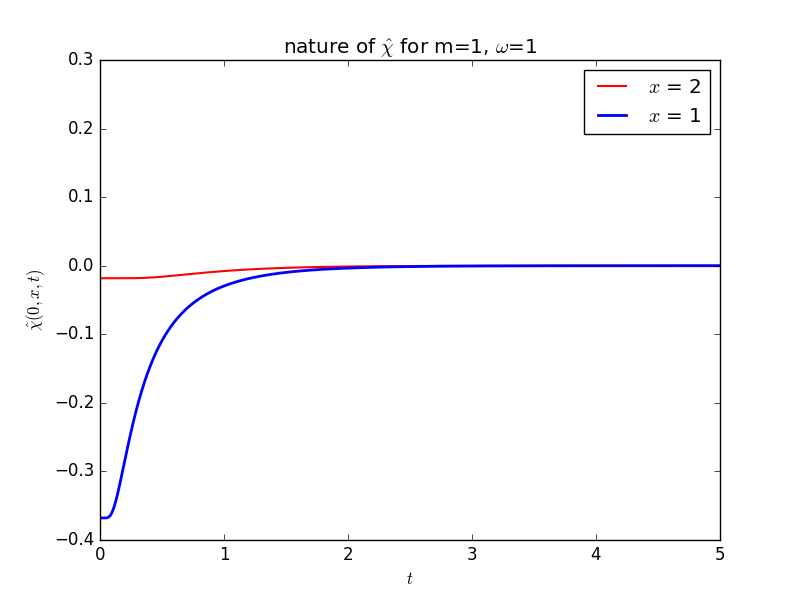
\includegraphics[scale=0.7]{plots/chi.png}
\caption{$\chi$ as a function of time for different choice of $x'$ when $x=0$.}
\end{center}
\end{figure}
\subsection{Interpretation of 1D response function}
We now would try to interprete Eq.~\eqref{1d_chi}. To do that first let us parametrize
\eq
 \zeta(t)= \cos \theta(t)
\qe 
such that 
\eq
 \theta(t) = \cos^{-1} (e^{-\hbar \omega \abs{t}})
\qe
 With this parametrization, we can see Eq.~\eqref{1d_chi} takes the form 
\eq\label{1d_chi_theta}
\hat{\chi}(y, y', t)=-\sqrt{2\pi}\left( \frac{m \omega}{\pi \hbar}\right) \left(\left. \frac{e^{-\left(\frac{(\mathbf{y}'-\mathbf{y})^{2}}{\sin^2 \theta}\right)}}{\sin \theta}\right \rvert_{\theta=\theta(t)}- \left. \frac{e^{-\left(\frac{(\mathbf{y}'-\mathbf{y})^{2}}{\sin^2 \theta}\right)}}{\sin \theta} \right \rvert_{\theta=\pi/2}\right)
\qe
or 
\eq
\hat{\chi}(y, y', t)= K(y, y', \theta(t))- K(y, y', \pi/2)
\qe
where 
\eq
K(y, y', \theta(t)) = -\sqrt{2\pi}\left( \frac{m \omega}{\pi \hbar}\right) \left( \frac{e^{-\left(\frac{(\mathbf{y}'-\mathbf{y})^{2}}{\sin^2 \theta}\right)}}{\sin \theta}\right)
\qe
Here the vectors $\mathbf{y}'$ and $\mathbf{y}$ are defined in an "interaction" space whose length is $y'$ and $y$. They do not have any interaction (\ie they are independent) when $\theta = \pi/2$. So whenever there is an external source, they are "forced" to be squeezed at $\theta < \pi/2$. However, once released, they relax to $\theta = \pi/2$ with time. This is similar to spin-spin relaxation in NMR and vector $\mathbf{y}'$ and $\mathbf{y}$ are similar to Bloch vectors. The quantity $P(t) = \sin \theta(t)$ is the survival probability of the convolutions of the interacting state at time $t$ which behaves like the standard deviation for the normal distribution \textbf{\emph{(I am not sure what does that mean? This process can be understood in terms of Stat mech ?)}}. 

The process can be visualized as 

\begin{figure}[H]
\begin{center}
 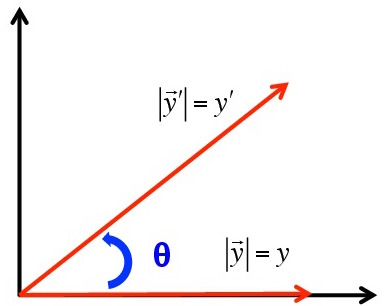
\includegraphics[scale=0.5]{plots/1D_Relaxation.jpg}
\caption{Relaxation of $\mathbf{y}'$ with respect to $\mathbf{y}$ with time.}
\end{center}
\end{figure}
The evolution of angle with time looks like :
\begin{figure}[H]
\begin{center}
 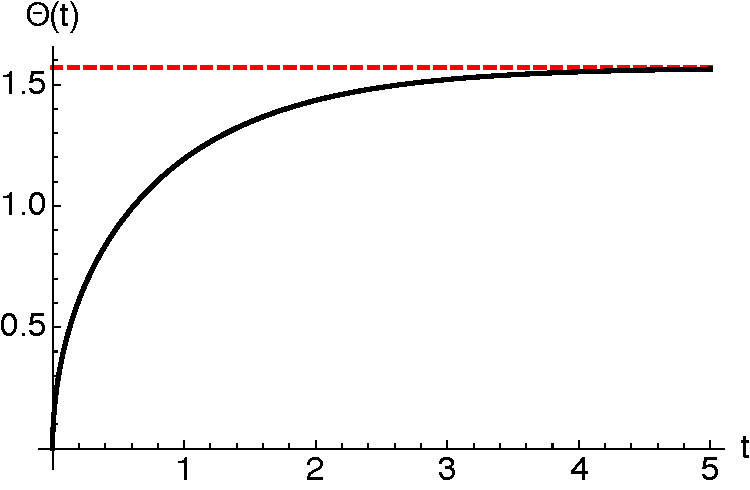
\includegraphics[scale=0.7]{plots/AngleEvolution.pdf}
\caption{Evolution of $\theta(t)$ with time. Red dashed line is $\pi/2$}
\end{center}
\end{figure}
The survival probability of "correlated" states looks like
\begin{figure}[H]
\begin{center}
 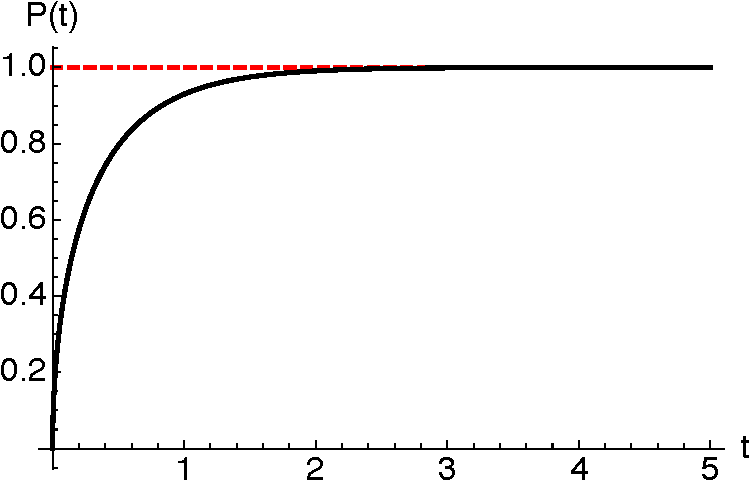
\includegraphics[scale=0.7]{plots/Survivalprobability.pdf}
\caption{Evolution of survival probability with time.Red dashed line is 1}
\end{center}
\end{figure}
One of the exact nature of response function will be that it will not be able to distinguish between uniform, homogeneous backgrounds. In other words, if the overall background potential changes by a constant amount, there will be no deformation in the shape of electron density. Mathematically it implies 
\eq\label{chg_neutral}
\int_{-\infty}^{\infty} \diff y' \hat{\chi}(y, y', \zeta) = 0
\qe
We will now see what our response function does.\\
To start with let us say
\begin{eqnarray}
A &=& -\sqrt{2\pi} \left( \frac{m \omega}{\pi \hbar}\right) \\
\beta &=& \frac{1}{\sqrt{1-\zeta^2}} \\
\alpha &=& \zeta y
\end{eqnarray}
Now
\eq\label{chi_int}
\int_{-\infty}^{\infty} \diff y' \hat{\chi}(y, y', \zeta) =\int_{-\infty}^{\infty} \diff y' K(y, y', \zeta) -\int_{-\infty}^{\infty} \diff y' K(y, y', 0) 
\qe
The first term in Eq.~\eqref{chi_int} is 
\eq
\int_{-\infty}^{\infty} \diff y' K(y, y', \zeta) = A \beta \int_{-\infty}^{\infty} \diff y' e^{-\beta^2(y^2+{y'}^2- 2\alpha y')} 
\qe
Completing the square with $y'$ the right hand side of above equation becomes 
\eq
\int_{-\infty}^{\infty} \diff y' K(y, y', \zeta) = A \beta  e^{-\beta^2 y^2} e^{\beta^2 \alpha^2}\frac{\sqrt{\pi}}{\beta}=A\sqrt{\pi} e^{-{y}^2}
\qe
Since the result is independent of $\zeta$, the second term in Eq.~\eqref{chi_int} will yield the same term. As a result, Eq.~\eqref{chg_neutral} is satisfied. 

Now we will try to see if we can derive the expression for $\chi(y, y', u=0)$. We will start from deceptively simple looking Eq.~\eqref{chi_u} by setting $u = 0$.
\eq\label{chi_u0}
 \chi(x, x', i u=0)= -2\rho_{0}(x, x') \sum_{\mu=1}^{\infty}\rho_{\mu}(x, x')\left( \frac{1}{\mu \hbar \omega} \right)
\qe
or, 
\eq\label{chi_u0_full}
 \chi(y, y', i u=0)= -\frac{2}{\hbar \omega}\left( \frac{m \omega}{\pi \hbar}\right) e^{-(y^2+{y'}^2)} \sum_{\mu=1}^{\infty}\frac{H_{\mu}(y)H_{\mu}(y')}{2^{\mu}\fact{\mu}}\left( \frac{1}{\mu} \right)
\qe
Now we realize that 
\eq
\frac{\partial H_{\mu}(y)}{\partial y} = 2 \mu H_{\mu-1}(y)
\qe
or,
\eq
H_{\mu}(y) = 2\mu \int \diff y H_{\mu - 1}(y)
\qe
Therefore, 
\eq\label{chi_u0_wint}
 \chi(y, y', i u=0)= -\frac{2}{\hbar \omega}\left( \frac{m \omega}{\pi \hbar}\right) e^{-(y^2+{y'}^2)} \iint \diff y \diff y' \sum_{\mu=1}^{\infty}\frac{2 H_{\mu-1}(y)H_{\mu-1}(y')}{2^{\mu-1}\fact{(\mu-1)}}
\qe
Changing the dummy index limit by $(\mu -1) \rightarrow \mu$
\eq\label{chi_u0_wint2}
 \chi(y, y', i u=0)= -\frac{4}{\hbar \omega}\left( \frac{m \omega}{\pi \hbar}\right) e^{-(y^2+{y'}^2)} \iint \diff y \diff y' \sum_{\mu=0}^{\infty}\frac{H_{\mu}(y)H_{\mu}(y')}{2^{\mu}\fact{\mu}}
\qe
However we know that 
\eq
\sum_{\mu=0}^{\infty}\frac{H_{\mu}(y)H_{\mu}(y')}{2^{\mu}\fact{\mu}} =\sqrt{\pi}  e^{\frac{y^2+{y'}^2}{2}}\delta(y-y')
\qe
Therefore, the expression becomes 
\eq\label{chi_u0_wint3}
 \chi(y, y', i u=0)= -\frac{4\sqrt{\pi}}{\hbar \omega}\left( \frac{m \omega}{\pi \hbar}\right) e^{-(y^2+{y'}^2)} \iint \diff y \diff y' e^{\frac{y^2+{y'}^2}{2}}\delta(y-y')
\qe
\textbf{\emph{Note that the integrals here are indefinite integrals ! We better be careful here. We may not be able to use the beautiful properties of Delta functions here easily. Needs thoughts and very careful analyses. }}

We may advance a bit more: We know
\eq
\lim_{a \to \infty}\sqrt{\frac{a}{\pi}}e^{-a x^2} \equiv \delta(x)
\qe

Therefore, 
%\label{deltaexp}
\eq
\chi(y, y', i u=0)= -\left( \frac{4m}{\pi \hbar^2}\right) e^{-(y^2+{y'}^2)} \lim_{a \to \infty} \sqrt{a} \iint \diff y \diff y' e^{\frac{y^2+{y'}^2}{2}}e^{-a(y-y')^2}
\qe
Going to collective coordinates
\begin{eqnarray}\label{collcoord_y}
z &=& \frac{y+y'}{\sqrt{2}}\\
z' &=&  \frac{y-y'}{\sqrt{2}}
\end{eqnarray}

%we can rewrite Eq.\eqref{deltaexp} as 

\eq
\chi(y, y', i u=0)= -\left( \frac{4m}{\pi \hbar^2}\right) e^{-(y^2+{y'}^2)} \lim_{a \to \infty} \sqrt{a} \iint \diff z \diff z' e^{z^2}e^{{z'}^2 \lp 1-2a\rp}
\qe

Now we will explore the spatial variation of the response function. Below we see how $\hat{\chi}(y, y',t)$ evolves with time. We can see the density responds diffrently depending on the absolute position of cause and effect leading to positive and negative points in the plot. This is in accordance to the Eq.~\eqref{chg_neutral}. Spatial inhomogeneity of $\hat{\chi}(y, y',t)$ also decreases with time indicating a damping and "spreading of disturbance". It is clear that the effect of fluctuation is large locally while the response is quite delocalized indicating long-range correlations.
Now this is road block ! However if we are allowed to analytically continue the $\{y, y'\}$ domain, for $z \rightarrow i z $ and $z' \rightarrow i z' $ we get 
\eq
\chi(iy, iy', iu = 0) = \lp\frac{4im}{\sqrt{2}\pi \hbar^2} \rp e^{(y^2+{y'}^2)}\erf\lp {\frac{y+y'}{\sqrt{2}}}\rp \lim_{a \to \infty} \erf\lp\lp y-y' \rp\sqrt{1/2-a}\rp
\qe
Here we used 
\eq
\lim_{a \to \infty}\sqrt{\frac{a}{1-2a}} = \frac{i}{\sqrt{2}} 
\qe
However, nothing significant came ! 
\begin{figure}[H]
\begin{center} 
   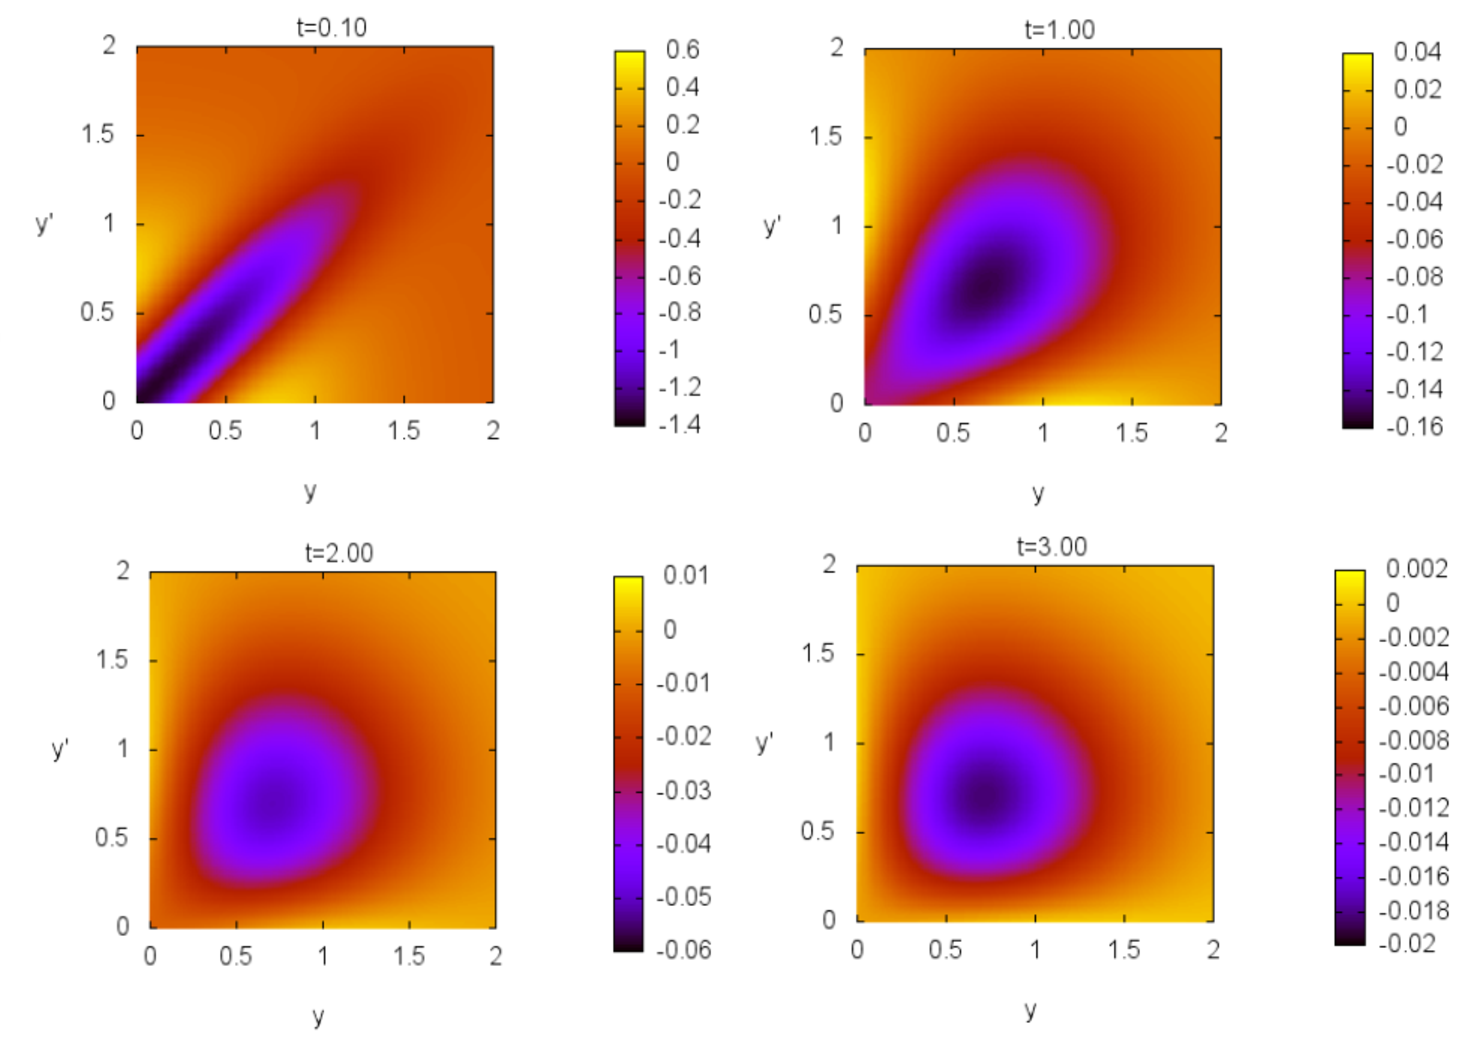
\includegraphics[scale=0.4]{plots/Plotpanel1.pdf} 
  \caption{Evolution of $\hat{\chi}$ : Early phase}
  \label{Panel1}
 \end{center}
\end{figure}  
\begin{figure}[H]
\begin{center}
   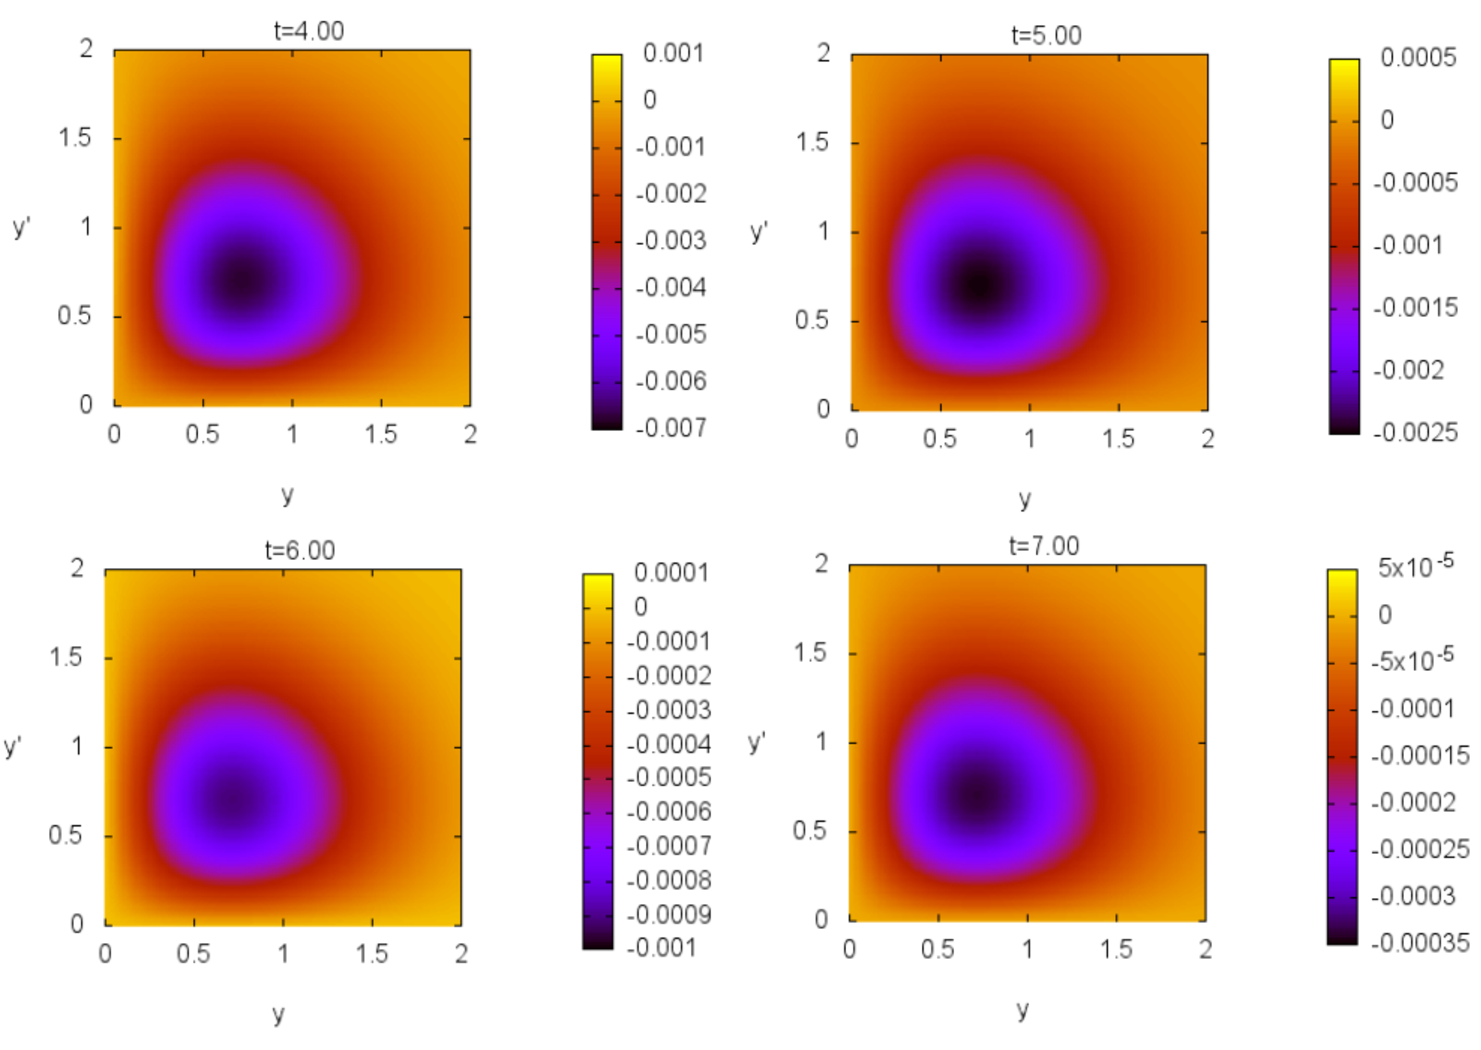
\includegraphics[scale=0.4]{plots/Plotpanel2.pdf} 
  \caption{Evolution of $\hat{\chi}$ : Middle phase}
  \label{Panel2}
 \end{center}
\end{figure}  
\begin{figure}[H]
\begin{center}
   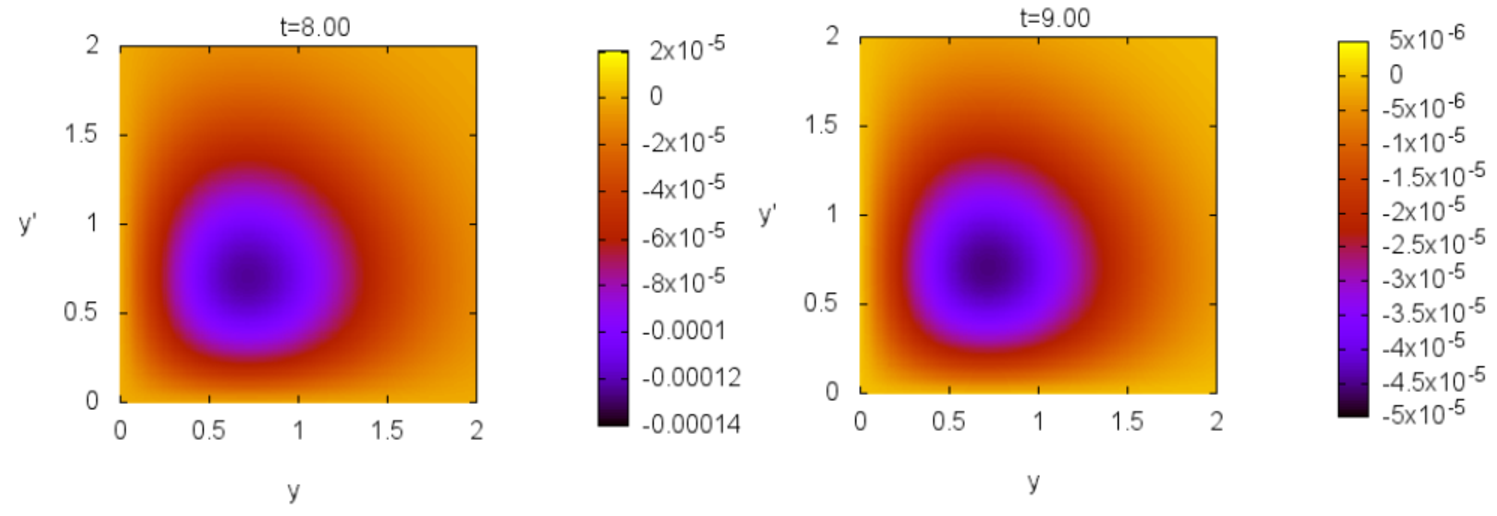
\includegraphics[scale=0.4]{plots/Plotpanel3.pdf} 
  \caption{Evolution of $\hat{\chi}$ : Late phase}
  \label{Panel3}
 \end{center}
\end{figure}  

Interestingly the minimum of $\hat{\chi}$ apparently starts from near $y=y'=0$ and moves away fast in the early phase (Fig.~\ref{Panel1}) of evolution. However we see it stops there at later periods (Fig.~\ref{Panel2} and Fig.~\ref{Panel3}). To analyse that we follow the evolution of minimum of $\hat{\chi}(y, y'=y, t)$ below. We find that 
\eq
\frac{\partial \hat{\chi}(y, y, t)}{\partial y} = 0
\qe
is satisfied for either
\eq
y_{crit}=0
\qe
or
\eq\label{ymin}
y_{crit}= \left[ \left(\frac{1+\zeta(t)}{2\zeta(t)}\right) \ln((1+\zeta(t))\sqrt{1-\zeta^2(t)})\right]^{1/2}
\qe
The first critical point is a saddle point in longer time while the second is a minimum/maximum in longer time depending on the parity of $y y'$.
Time evolution of $y_{crit} = y_{min}$ in Eq.~\eqref{ymin} is plotted below. Clearly we see $y_{min}$ converges to a value close to 0.71(red dashed line) which matches with the Figs.~(\ref{Panel1}, \ref{Panel2}, \ref{Panel3}). 
\begin{figure}[H]
\begin{center}
   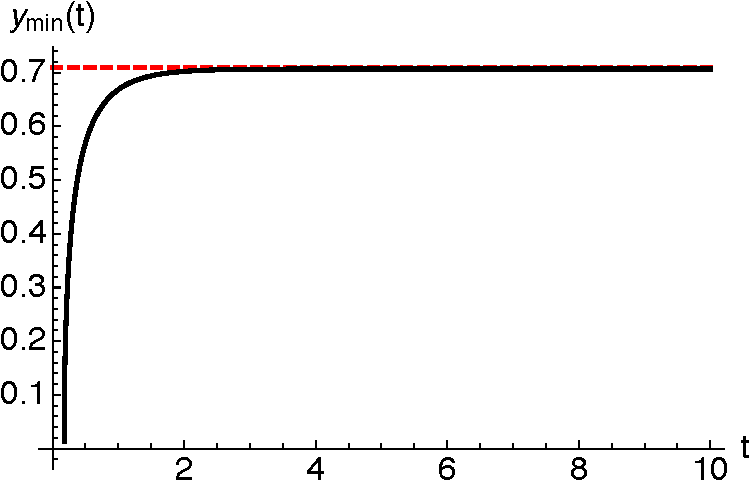
\includegraphics[scale=0.7]{plots/Yminevolution.pdf} 
  \caption{Evolution of minimum of $\hat{\chi}$}
  \label{ymin}
 \end{center}
\end{figure}  
This minimum appears for time $t \geq t_{crit}$ where critical time  $t_{crit}$ is the solution of 
\eq
(1+\zeta(t))\sqrt{1-\zeta^2(t)} = 1
\qe
Clearly there are four possible solutions of it. \textbf{WHY?}
\subsection{Effect of evolution of critical points in correlation energy}
\textbf{To be done}
\subsection{$\chi$ in truncated basis}
\textbf{To be done}
\subsection{Polarizability of 1D SHO}
 We have relation between polarizability $\alpha(y, y')$ and $\chi (y, y')$ as
\eq\label{1dchi_alpha}
\frac{\partial^2}{\partial y \partial y'}\alpha(y, y') = \chi(y, y').
\qe
This relation is valid for both time and frequency dependent response functions. Therefore
\eq\label{1dchi_alphat}
 \frac{\partial^2}{\partial y \partial y'}\alpha(y, y', t) =\hat{\chi}(y, y', t)
\qe
Using Eq.\eqref{collcoord_y}, we can write
\eq
\hat{\chi}(z, z', t) = -C\left[ \frac{e^{-\frac{z^2}{1+\zeta(t)}}e^{-\frac{{z'}^2}{1-\zeta(t)}}}{\sqrt{1-\zeta^2(t)}} - e^{-z^2}e^{-{z'}^2}\right]
\qe
where $C = \sqrt{2\pi}\lp \frac{m \omega}{\pi \hbar} \rp$ and $\zeta(t) = e^{-\hbar \omega \abs{t}}$. In this collective coordinate, we can now express Eq.\eqref{1dchi_alpha} as 
\eq
\lp \frac{\partial^2}{\partial z^2} - \frac{\partial^2}{\partial {z'}^2}\rp \alpha(z, z', t)= 2 \hat{\chi}(z, z', t)
\qe
Using Fourier transform we obtain
\eq\label{chik}
\begin{split}
 \tilde{\chi}(\kappa, \kappa', t) &= \frac{1}{2 \pi} \int_{-\infty}^{\infty} \diff z e^{i \kappa z}\int_{-\infty}^{\infty} \diff z' e^{i \kappa' z'} \hat{\chi}(z, z', t)\\
 &= -\frac{C}{2}\lp e^{-\frac{\kappa^2}{4 \sigma_1}}e^{-\frac{\kappa'^2}{4 \sigma_2}} - e^{-\frac{\kappa^2}{4}}e^{-\frac{\kappa'^2}{4}}\rp
\end{split}
\qe
where
\begin{eqnarray}
\sigma_1 &=& \frac{1}{\sqrt{1+\zeta(t)}}\\
\sigma_2 &=& \frac{1}{\sqrt{1-\zeta(t)}}
\end{eqnarray}
 and the expression of $\tilde{\alpha}(\kappa, \kappa', t)$ as 
\eq\label{alpha_pm}
\tilde{\alpha}(\kappa, \kappa', t) = 2 \frac{\tilde{\chi}(\kappa, \kappa', t)}{\lp {\kappa'}^{2} -\kappa^2\rp}
\qe
Therefore  using convolution theorem 
\eq
\alpha(z, z', t) = \int_{-\infty}^{\infty} \diff s \int_{-\infty}^{\infty} \diff s' \hat{\chi}(s, s',t) g(z-s, z'-s', t)
\qe
where 
\eq
g(s, s', t) = \frac{1}{2 \pi} \int_{-\infty}^{\infty} \diff \kappa e^{-i \kappa s}\int_{-\infty}^{\infty} \diff \kappa' e^{-i \kappa' s'} \frac{1}{{\kappa'}^{2}-\kappa^{2}}
\qe
Alternatively we can try to use complex integration to directly calculate $\alpha(z, z',t)$ from Eq.\eqref{alpha_pm}. However that gives disastrous result as follows ! 
\eq
\alpha(z, z', t) = \lp\frac{1}{2\pi}\rp \int_{-\infty}^{\infty}\diff \kappa e^{-i\kappa z}\int_{-\infty}^{\infty}\diff \kappa' e^{-i\kappa' z'}\tilde{\alpha}(\kappa, \kappa', t) 
\qe
or,
\eq
\alpha(z, z', t) = \lp\frac{1}{\pi}\rp \int_{-\infty}^{\infty}\diff \kappa \frac{e^{-i\kappa z}}{2\kappa}\int_{-\infty}^{\infty}\diff \kappa' e^{-i\kappa' z'} \tilde{\chi}(\kappa, \kappa', t)\lp \frac{2\kappa}{{\kappa'}^{2} -\kappa^2}\rp
\qe
or, 
\eq
\alpha(z, z', t) = \lp\frac{1}{2\pi}\rp \int_{-\infty}^{\infty}\diff \kappa \frac{e^{-i\kappa z}}{\kappa}\int_{-\infty}^{\infty}\diff \kappa' e^{-i\kappa' z'} \tilde{\chi}(\kappa, \kappa', t)\lp \frac{1}{\kappa' -\kappa}-\frac{1}{\kappa' + \kappa}\rp
\qe
Using Residue theorem, 
\eq
\alpha(z, z', t) =  i \int_{-\infty}^{\infty}\diff \kappa \frac{e^{-i\kappa z}}{\kappa} \left[ e^{-i\kappa z'} \tilde{\chi}(\kappa, \kappa, t)- e^{i\kappa z'} \tilde{\chi}(\kappa, -\kappa, t)\right]
\qe
We know from Eq.\eqref{chik}
\eq
\tilde{\chi}(\kappa, \kappa, t)=\tilde{\chi}(\kappa, -\kappa, t)
\qe
Therefore, 
\eq
\alpha(z, z', t) =  2 \int_{-\infty}^{\infty}\diff \kappa \frac{e^{-i\kappa z}}{\kappa} \sin(k z')  \tilde{\chi}(\kappa, \kappa, t)
\qe
or, 
\eq
\alpha(z, z', t) =  -i \lim_{\epsilon \to 0}  \lp\int_{-\infty}^{\infty}\diff \kappa\tilde{\chi}(\kappa, \kappa, t) \frac{e^{i\kappa (z-z')}}{(\kappa-i\epsilon)}  - \int_{-\infty}^{\infty}\diff \kappa\tilde{\chi}(\kappa, \kappa, t) \frac{e^{-i\kappa (z+z')}}{(\kappa-i\epsilon)}\rp
\qe
or,
\eq
\alpha(z, z', t) =  2\pi \lim_{\epsilon \to 0}  \tilde{\chi}(i\epsilon, i\epsilon, t) \lp e^{-\epsilon (z-z')}  - e^{-\epsilon (z+z')}\rp = 0
\qe
Clearly it is a problem with the normal mode transformation. Therefore we have to start from Eq.\eqref{1dchi_alphat}. The Fourier-transformed Eq.\eqref{1dchi_alphat} is 
\eq
- \kappa \kappa' \tilde{\alpha}(\kappa, \kappa', t) = \tilde{\chi}(\kappa, \kappa', t)
\qe
Note that here 
\eq
\tilde{\chi}(\kappa, \kappa', t) = \lp \frac{1}{2 \pi} \rp \int_{-\infty}^{\infty} \diff y e^{i \kappa y}\int_{-\infty}^{\infty} \diff y' e^{i \kappa' y'} \hat{\chi}(y, y', t)
\qe
and is different from Eq.\eqref{chik}. The real space polarizability kernel is then
\eq
\alpha(y, y', t) = \lp \frac{-1}{2\pi}\rp \int_{-\infty}^{\infty} \diff \kappa e^{-i \kappa y}\int_{-\infty}^{\infty} \diff \kappa' e^{-i \kappa' y'} \frac{\tilde{\chi}(\kappa, \kappa', t)}{\kappa \kappa'}
\qe
Before we go any further, we note two relations we believe will be important.
\eq\label{ft_xinv}
\int_{-\infty}^{\infty} e^{i\kappa x} \frac{1}{ x} \diff x = -i \pi \sign(\kappa)
\qe
and 
\eq\label{ft_exp}
\int_{-\infty}^{\infty} e^{i\kappa x} e^{-b(x^2 - 2c x)} \diff x = \sqrt{\frac{\pi}{b}} e^{\lp-\frac{\kappa^2}{4b} + bc^2 + i\kappa c\rp}
\qe

Here the sign function is defined as 
\eq
\sign(x) = \threepartdef { -1} {x < 0} {0} {x = 0} {1} {x>0} 
\qe
\footnote{There is a relation between half-maximum Heaviside theta function $\Theta(x)$ and $\sign(x)$: $\sign(x) = 2\Theta(x)-1$}
Now the half Fourier transformed response function is 

\eq
 \chi'(\kappa, y', t) = \frac{1}{\sqrt{2\pi}}\int_{-\infty}^{\infty} e^{i\kappa y} \hat{\chi}(y, y', t)\diff y
\qe
Using $\gamma = \frac{1}{\sqrt{1-\zeta^2(t)}}$, we can write
\eq
 \hat{\chi}(y, y', t) = -C\left[ \gamma e^{-\gamma^2 \lp y^{2}+{y'}^{2}-2\zeta(t)yy'\rp} -e^{-(y^2+{y'}^{2})}\right]
\qe
Therefore, 
\eq
 \chi'(\kappa, y', t) = \frac{-C}{\sqrt{2\pi}}\left[ \gamma e^{-\gamma^2 {y'}^{2}}\int_{-\infty}^{\infty} \diff y e^{i\kappa y} e^{-\gamma^2 \lp y^2 -2\zeta(t) y y'\rp} -e^{-{y'}^2}\int_{-\infty}^{\infty} \diff y e^{i\kappa y} e^{-y^2} \right]
\qe
or,
\eq
 \chi'(\kappa, y', t) = \frac{-C}{\sqrt{2\pi}}\left[ \gamma e^{-\gamma^2 {y'}^{2}} \sqrt{\frac{\pi}{\gamma^2} }e^{-\frac{\kappa^2}{4\gamma^2} + (\gamma \zeta(t)y')^2+ i\kappa y' \zeta(t)} -e^{-{y'}^2} \sqrt{\pi} e^{-\frac{\kappa^2}{4} } \right]
\qe
or,
\eq
 \chi'(\kappa, y', t) = \frac{-C}{\sqrt{2}}\left[  e^{-\gamma^2 {y'}^{2}} e^{-\frac{\kappa^2}{4\gamma^2} + (\gamma \zeta(t)y')^2+ i\kappa y' \zeta(t)} -e^{-{y'}^2}  e^{-\frac{\kappa^2}{4} } \right]
\qe
or, 
\begin{eqnarray}
\chi'(\kappa, y', t) &&= \frac{-C}{\sqrt{2}}e^{-{y'}^{2}} \left[  e^{-\frac{\kappa^2}{4\gamma^2} + i\kappa y' \zeta(t)} -  e^{-\frac{\kappa^2}{4} } \right]\\
&& = \frac{-C}{\sqrt{2}} \left[  e^{-\lp \lp y'-\frac{i\kappa \zeta(t)}{2} \rp^{2}+ \frac{\kappa^2}{4}\rp} -  e^{- \lp {y'}^{2}+\frac{\kappa^2}{4}\rp } \right]
\end{eqnarray}

Therefore, 
\begin{eqnarray}
&&\alpha(y, y', t) = \lp \frac{-1}{2\pi}\rp \int_{-\infty}^{\infty} \diff \kappa \frac{e^{-i \kappa y}}{\kappa}\int_{-\infty}^{\infty} \diff \kappa' e^{-i \kappa' y'} \frac{\tilde{\chi}(\kappa, \kappa', t)}{\kappa'}\\
     && =\lp \frac{-1}{\sqrt{2\pi}}\rp \int_{-\infty}^{\infty} \diff \kappa \frac{e^{-i \kappa y}}{\kappa}\lp \frac{1}{\sqrt{2\pi}}\rp\int_{-\infty}^{\infty} \diff \kappa' e^{-i \kappa' y'} \frac{\tilde{\chi}(\kappa, \kappa', t)}{\kappa'}\\
 &&= \lp \frac{1}{\sqrt{2\pi}}\rp \int_{-\infty}^{\infty} \diff \kappa \frac{e^{-i \kappa y}}{\kappa} \lp \frac{i \pi}{\sqrt{2\pi}}\rp \int_{-\infty}^{\infty} \diff s \sign(y'-s) \chi'(k, s, t)
\end{eqnarray}
Together, 
\eq
\alpha(y, y', t) = \lp \frac{i}{2}\rp \int_{-\infty}^{\infty} \diff \kappa \frac{e^{-i \kappa y}}{\kappa}  \int_{-\infty}^{\infty} \diff s \sign(y'-s) \chi'(k, s, t)
\qe
With a bit of little algebra and using definitions of error functions, we arrive at 
\eq
\alpha(y, y', t) = \lp \frac{iC}{4}\rp \left[ \erf(y') \int_{-\infty}^{\infty} \diff \kappa \frac{e^{-i \kappa y}}{\kappa} e^{-\frac{\kappa^2}{4}}  - \int_{-\infty}^{\infty} \diff \kappa \frac{e^{-i \kappa y}}{\kappa} e^{-\frac{\kappa^2}{4}} \epsilon \lp y',k \rp \right]
\qe
where 
\eq
\epsilon \lp y', k\rp = \frac{2}{\sqrt{\pi}} \int_{-y'}^{y'} e^{-(s-\frac{ik\zeta(t)}{2})^{2}} \diff s 
\qe
as a result,
\eq
\alpha(y, y', t) = \lp \frac{iC}{4}\rp \left[ \erf(y') \varphi(y) - \int_{-\infty}^{\infty} \diff \kappa \frac{e^{-i \kappa y}}{\kappa} e^{-\frac{\kappa^2}{4}} \epsilon \lp y',k \rp \right]
\qe
where,
\eq
\varphi(y) = \int_{-\infty}^{\infty} \diff \kappa \frac{e^{-i \kappa y}}{\kappa} e^{-\frac{\kappa^2}{4}}=\lp {i\sqrt \frac{\pi}{2}} \rp \erf(y)
\qe
Using convolution theorem, 
\eq
\alpha(y, y', t) = \lp \frac{iC}{4}\rp \left[ \erf(y') \varphi(y) - \int_{-\infty}^{\infty} \diff s \varphi(y-s) \tilde{\epsilon} (y',s) \right]
\qe
where 
\eq
\tilde{\epsilon}(y', y) =\mathcal{F}^{-1}[\epsilon(y', k)]
\qe

\textbf{Clearly, the first term inside square bracket is symmetric under exchange of $y$ and $y'$. An educated guess indicates the second term will be reduced to the first term upto a numerical constant as $t \to \infty, \zeta \to 0$. }

\subsection{Response function for 3D isotropic oscillator}
 The wavefunction and energy of a 3D oscillator are given by Eq.~\eqref{shof} and Eq.~\eqref{3den}, respectively. The corresponding AWS now defines the 3D response function of the 3D oscillator. \\

\emph{We now realize that the ground state is nondegenerate which guarantees that for $\mu = 0$, $\mu_{x} = \mu_{y} = \mu_{z} = 0$ has to satisfy.} 
\eq
f_{\mu} = \delta_{\mu_{x}0}\delta_{\mu_{y}0}\delta_{\mu_{z}0}
\qe
  Now comes the crux of the solution. \emph{The sums in Eq.~\eqref{awsum} runs from $0$ to $\infty$. Let us create a list of $\mu$ in $[0,\infty]$. Each element $\mu$ again can be partitioned in three integers $\mu_{x}$, $\mu_{y}$ and $\mu_{z}$. This procedure creates a list of strings of three numbers where each number appears only once and the full list contains all possible combinations of three positive integers, }
\eq
\sum_{\mu= \mu_{x}+\mu_{y}+\mu_{z}= 0}^{\infty} \equiv \sum_{\mu_{x}=0}^{\infty}\sum_{\mu_{y}=0}^{\infty}\sum_{\mu_{z}= 0}^{\infty} 
\qe
 \emph{ \ie the \textbf{sum over $\mu $ tantamounts to independently summing over $\mu_{x}$, $\mu_{y}$ and $\mu_{z}$.}} Therefore, for 3D isotropic oscillator the AWS becomes
\eq
\chi_{3D}(\rr, \rr',i u) = \sum_{\mu_{x},\mu_{y},\mu_{z} = 0}^{\infty}  \sum_{\nu_{x},\nu_{y},\nu_{z} = 0}^{\infty} \frac{(f_{\mu}-f_{\nu})\rho_{\mu}(\rr, \rr')\rho_{\nu}(\rr, \rr')}{(\mu-\nu)\hbar\omega + i u}
\qe 
Using the same prescription of 1D case, we obtain the time domain response function as 
\eq
\begin{split}
\hat{\chi}_{3D}(\rr, \rr', t)& =-\sqrt{2\pi} \lp\frac{m \omega}{ \pi\hbar}\rp^{3} e^{-\frac{m\omega(\rr^2+\rr'^2)}{\hbar}} \\
&\times \left( \sum_{\mu_{x},\mu_{y},\mu_{z} = 0}^{\infty} \frac{\prod_{i = x}^{z}H_{\mu_{i}}(\sqrt{m \omega} i)H_{\mu_{i}}(\sqrt{m \omega} i')e^{-\mu_{i}\omega\hbar\abs{t}}}{2^{\mu}\prod_{i = x}^{z}\mu_{i}!} - 1\right)
\end{split}
\qe
The unity in the last parenthesis stems from the fact that for $\mu=\nu=0$ the AWS vanishes identically. Since the sums are independent, we now can write
\eq
\hat{\chi}_{3D}(\rr, \rr', t) = \tilde K(\rr, \rr', \theta(t))- \tilde K(\rr, \rr', \pi/2)
\qe
where 
\eq
  \tilde K(\rr, \rr', \theta(t))= K(x, x', \theta(t)) K(y, y', \theta(t)) K(z, z', \theta(t))
\qe
We can see this response function also goes to zero for $t \rightarrow \infty$ and vanishes when integrated over $\rr'$. However for a nonspherical potential (say $x$-directional) it shows a density deformation in all directions.  
\section{Response function of ``1D H atom''}
The solution of 1D H-atom (taken from A. N. Gordeyevy and S C Chhajlanyz, \emph{J. Phys. A: Math. Gen}, \textbf{30}(1997)6893)
\eq
\frac{\diff^2 \psi}{\diff x^2} -\left( \lambda - \frac{\alpha}{\abs{x}}\right) = 0
\qe 
is 
\eq
\psi_{n} = B_{n} x L_{n}^{1}(\beta_{n}\abs{x})e^{\left(-\frac{\beta_{n}\abs{x}}{2}\right)}
\qe
where 
\eq
\beta_n = \frac{\alpha}{n+1},
\qe
$B_n$ is normalization factor and $L_{n}^{1}$ is associated Lauguerre polynomial. 
The energy is
\eq
E_n= -\frac{m e^4}{2 \hbar^2(n+1)^2}
\qe
Here we used $\lambda = 2m\abs{E}/\hbar^2$, $\alpha = 2m e^2/\hbar^2$ and $E = -\abs{E}$. 

\begin{appendices}
\section{Complex analysis}

This section will be a quick sammary of ideas and expressions of complex analysis. We will, probabaly, need it to go through the mathematics of response functions.
\subsection{Complex functions}
 A complex function is a function $\chi(x+iy) = u(x,y) + i v(x,y)$ where $u, v: \mathbb{R}^{2}\rightarrow \mathbb{R}$ such that $\chi: \mathbb{R}\times\mathbb{R}\rightarrow \mathbb{C} $ and $x, y \in \mathbb{R}$. The complex variable $z = x +iy$ is a point in complex plane.  
\subsection{Complex differentiation}
A complex function $\chi(z)$ is differentiable at point $z_{0}$ in complex plane if the limit
\eq
\lim_{z \to z_{0}}\frac{\chi(z)-\chi(z_{0})}{z-z_{0}}
\qe
exists and the limiting value $\chi'(z_{0})$ will be called the \emph{derivative} of $\chi(z)$ at $z_{0}$.\\

\textbf{Cauchy-Riemann condition}\\
The conditions for a function $f(z) = u(x,y) + i v(x, y)$ to be differentiable around point $z_{0}$ are called Cauchy-Riemann conditions: 
\begin{eqnarray}
 \frac{\partial u}{\partial x} =  \frac{\partial v }{\partial y } \\
 \frac{\partial{v}}{\partial{x}}= -\frac{\partial{u}}{\partial{y}}
\end{eqnarray}
\begin{itemize}
\item A function that is infinitly-differentiable in the neighbourhood of point $z_{0}$ is called \emph{holomorphic} functions. Holomorphic functions are also \emph{analytic} as it can be expressed as a convergent power series around $z_{0}$ and is equal to its Taylor-series. 
\item A function which is holomorphic in its entire domain is called \emph{entire} function
\end{itemize}
\subsection{Complex integration}
Integration of a complex function $f(z)$ over a path $\gamma$ in the complex plane is defined as 
\eq
 \int_{\gamma} f(z) \diff z = \int_{a}^{b} \diff t f(\gamma(t))\gamma'(t) 
\qe
The integration path $\gamma$ is parametrized here. 
\begin{definition}
Suppose $\gamma_{0}$ and $\gamma_{1}$ two closed paths in region $G \subseteq \mathbb{C}$ and parametrized by $\gamma_{0}(t), 0\leq t \leq1$ and $\gamma_{1}(t), 0 \leq t \leq1$, respectively.  $\gamma_{0}$ is G-\textbf{homotopic} to $\gamma_{1}$ if there exists a continuous function $h:[0, 1]^{2} \to G$ such that $\forall t, s \in [0, 1]$
 \begin{eqnarray}
   h(t, 0) &=& \gamma_{0}(t) \nonumber \\
   h(t, 1) &=& \gamma_{1}(t)\\
   h(0, s)&=& h(1,s) \nonumber
 \end{eqnarray}
This is the \textbf{"topological deformation of paths"}
\end{definition}

\begin{theorem}[Cauchy-Goursat theorem]
Suppose $f$ is a holomorphic function in $G\subseteq \mathbb{C}$ and two carves $\gamma_{0}$ and $\gamma_{1}$ are \textit{piecewise-smooth curves} in region $G$  and $\gamma_{0}$ is G-homotopic to $\gamma_{1}$. Then 
\eq
 \int_{\gamma_{0}} f = \int_{\gamma_{1}} f
\qe
\end{theorem}
Which means if the paths are topologically \emph{equivalent} the integration is independent of the choice of path.
\begin{corollary}
Let $U$ be an open subset of $\mathbb{C}$ which is simply connected and let $f : U \rightarrow \mathbb{C}$. Let $\gamma$ is a rectifiable closed path in $U$. Then
\eq
\oint_{\gamma} f(z) dz = 0
\qe 
\end{corollary}
Proof requires the applications of Cauchy-Riemann conditions and Greens theorem ($\oint_{\gamma} (L \diff x + M \diff y) = \iint_{D}\diff x \diff y (\frac{\partial M}{\partial x} -\frac{\partial L}{\partial y} ) $ where $D$ is the open region bounded by $\gamma$) on the holomorphic function $f(z) = u (x, y) + i v(x, y)$. 
\subsection{Isolated singularity and Laurent series}
If $f$ is a holomorphic function in a region $D\subseteq \mathbb{C}$ except a point $z_{0}$. In other words, if for a certian $z_{0} \in D$, $f(z) = (z-z_{0})^{m} g(z), m > 0$ and $g(z)$ is holomorphic in $D$ then $z_{0}$ is an isolated singularity. 

\begin{definition}[Laurent series]
 A Laurent series of a holomorphic function $f(z)$ around a point $z_{0}$ is defined by
\eq
f(z) = \sum_{k=-\infty}^{\infty} c_{k} (z-z_{0})^{k}
\qe
\end{definition}
 A Laurent series is the natural extension of Taylor series.  



\subsection{Cauchy integral formula}




\section{Interesting relation: needs checking}

If
\eq
J_{k}(x_1, x_2)= \sum_{m=0}^{\infty}\frac{m^k H_{m}(x_1)H_{m}(x_2)}{2^m m!}
\qe
then
\eq
J_{k+1}= \frac{1}{2}\frac{\partial^2}{\partial x_1 \partial x_2}\left[\sum_{r=0}^{k}\binom{k}{r}(-1)^{k-r} J_{r}\right] - J_{k}
\qe
 where 
\eq
J_{0} = e^{-\lp\frac{x_1^2 + x_2^2}{2}\rp} \delta(x_1-x_2)
\qe
\end{appendices} 

\end{document}
